%%%%%%%%%%%%%%%%%%%%%%% file typeinst.tex %%%%%%%%%%%%%%%%%%%%%%%%%
%
% This is the LaTeX source for the instructions to authors using
% the LaTeX document class 'llncs.cls' for contributions to
% the Lecture Notes in Computer Sciences series.
% http://www.springer.com/lncs       Springer Heidelberg 2006/05/04
%
% It may be used as a template for your own input - copy it
% to a new file with a new name and use it as the basis
% for your article.
%
% NB: the document class 'llncs' has its own and detailed documentation, see
% ftp://ftp.springer.de/data/pubftp/pub/tex/latex/llncs/latex2e/llncsdoc.pdf
%
%%%%%%%%%%%%%%%%%%%%%%%%%%%%%%%%%%%%%%%%%%%%%%%%%%%%%%%%%%%%%%%%%%%


\documentclass[runningheads,a4paper]{llncs}

% inserido por mim
\usepackage[utf8]{inputenc}
\usepackage[T1]{fontenc}
\usepackage{lmodern} % load a font with all the characters
\usepackage[portuguese]{babel}
\usepackage{color}
\usepackage{graphicx}

\usepackage{amssymb}
\setcounter{tocdepth}{3}
\usepackage{graphicx}

\usepackage{url}
\urldef{\mailsa}\path|j.campinhos@campus.fct.unl.pt,|
\urldef{\mailsb}\path|p.duraes@campus.fct.unl.pt|
\newcommand{\keywords}[1]{\par\addvspace\baselineskip\noindent\keywordname\enspace\ignorespaces#1}

\begin{document}

\mainmatter% start of an individual contribution

% first the title is needed
\title{Novas fronteiras da ética na Informática:\\Inteligência Artificial e Agentes Autónomos}

% a short form should be given in case it is too long for the running head
\titlerunning{Inteligência Artificial e Agentes Autónomos}

% the name(s) of the author(s) follow(s) next
%
% NB: Chinese authors should write their first names(s) in front of
% their surnames. This ensures that the names appear correctly in
% the running heads and the author index.
%
\author{João Campinhos e Pedro Durães}
%
\authorrunning{Inteligência Artificial e Agentes Autónomos}
% (feature abused for this document to repeat the title also on left hand pages)

% the affiliations are given next; don't give your e-mail address
% unless you accept that it will be published
\institute{Faculdade de Ciências e Tecnologia da Universidade Nova de Lisboa,\\
  Quinta da Torre, 2829 -- 516 Caparica, Portugal\\
  \mailsa\\
  \mailsb\\
\url{http://http://www.fct.unl.pt}}

%
% NB: a more complex sample for affiliations and the mapping to the
% corresponding authors can be found in the file "llncs.dem"
% (search for the string "\mainmatter" where a contribution starts).
% "llncs.dem" accompanies the document class "llncs.cls".
%

\toctitle{Inteligência Artificial e Agentes Autónomos}
\tocauthor{Inteligência Artificial e Agentes Autónomos}
\maketitle


\begin{abstract}
  Este documento visa analisar o tema da inteligência artificial e agentes autónomos no âmbito dos aspectos sócio-profissionais da informática.
  Iremos abordar não só a forma como a inteligência artificial pode ajudar a humanidade, mas também os problemas éticos e riscos que levanta.
  Com o desenvolvimento cada vez mais rápido da inteligência artificial, deparamo-nos com inúmeros riscos que podem levar à extinção da humanidade, se não forem propriamente ponderados.
  \keywords{ia, inteligência artificial, autónomos, super-inteligência, ética, evolução, fct}
\end{abstract}

\section{Introdução}

A inteligência artificial está muito associada a robôs pois este é um tema bastante abordado no cinema. Geralmente nesses filmes, os engenheiros que programam estes agentes autónomos criam algo maior que eles próprios e que deixam de poder controlar. Mas isto é ficção, e na verdade o nosso objectivo com este documento é tentar aproximar este tema da realidade, pois apesar de ainda estarmos numa fase bastante embrionária no desenvolvimento de agentes autónomos, é uma área potencialmente perigosa, e cabe-nos a nós, engenheiros e futuros engenheiros informáticos, com um desenvolvimento responsável fazer com que o mau da inteligência artificial nunca venha ao de cima.

Existe ainda uma certa relutância e negação quando é abordado este tema, pois para algumas pessoas, parece tão provável o desenvolvimento de um agente super-inteligente como uma invasão de vampiros. Na verdade, cada vez mais pessoas importantes na área estão a levá-lo a sério, como é o caso do Elon Musk, cofundador do Paypal e Tesla Motors e fundador da empresa de exploração espacial SpaceX, que doou 10 milhões de dólares para o instituto Future of Life Institute\cite{FLI}, numa tentativa de promover um desenvolvimento da inteligência artificial e agentes autónomos estritamente beneficiais para a humanidade. Bill Gates afirma que ``Não percebo como existem pessoas que não estão preocupadas com o assunto``\cite{gates} e também Stephen Hawking alerta ``O desenvolvimento da inteligência artificial pode ditar o fim da raça humana``\cite{hawking}.

E isto são apenas alguns exemplos de personalidades bastante relevantes na área preocupadas, mas as discussões sobre este tema já duram à vários anos na comunidade cientifica. Podemos estar muito mais perto de uma revolução da inteligência artificial do que imaginamos, ao ponto dos cientistas acreditarem que em apenas 20 anos podemos vir a ter inteligência artificial ao nível dos humanos.

\section{Tipos de inteligência artificial}

Começando agora por falar na inteligência artificial. Neste momento (Maio de 2015) temos inteligência artificial em diversos objectos do nosso dia-a-dia. Mas essa inteligência artificial acaba por ser apenas benéfica para nós sem qualquer tipo de problema. O maior problema ético será a quantidade de informação que esses sistemas guardam sobre nós\footnote{Neste caso estamo-nos a referir a empresas como a Google que guarda o nosso histórico de pesquisa e sites visitados e locais onde fomos, entre outros dados sensíveis}. Neste documento vamos um pouco mais à frente falar na inteligência artificial que está neste momento a ser desenvolvida e cujo seu aparecimento tem muito mais consequências para nós. Vamos então classificar os vários tipos de inteligência artificial.

\subsection{Inteligência artificial restrita}
O primeiro nível encontra-se em muitos dos objectos do nosso dia-a-dia. Este nível denomina-se por inteligência artificial restrita. Restrita porque consegue ser mais inteligente e eficiente que o ser humano em tarefas muito especificas.
Temos como exemplos disto os diferentes sistemas que controlam os veículos actuais em funções como a travagem ou injecção de combustível para o motor, nos telemóveis quando usamos um mapa e obtemos direcções, no email ao automaticamente seleccionar o que é spam, no serviço Google translate e muitos outros exemplos.

\subsection{Inteligência artificial geral}
O segundo nível compara a inteligência artificial ao nível do ser humano, ou seja, uma máquina que consiga realizar tarefas intelectuais assim como o nosso cérebro. Tarefas como raciocinar, resolver problemas, pensar abstractamente, compreender ideias complexas e a habilidade de aprender.

\subsection{Super-inteligência artificial}
O terceiro nível, a super-inteligência artificial, leva-a muito além da capacidade do cérebro humano a todos os níveis. Veremos mais à frente que a distancia do salto do segundo para o terceiro nível é praticamente nulo, visto que a evolução da inteligência artificial é exponencial. É também neste nível que se impõem questões de extrema importância em relação ao nosso papel como seres humanos nesse contexto.

\section{Evolução da inteligência artificial}

Como referido, actualmente temos inteligência artificial distribuída em pequenas tarefas nos dispositivos que utilizamos. Qual o caminho a percorrer para termos um software que se equipare às tarefas que o nosso cérebro desenvolve?

\subsection{Aumento do poder computacional}

Para comparar o número de cálculos por segundo(cps) entre o cérebro humano e um computador, primeiro temos de calcular a capacidade do cérebro. Isto pode ser feito pegando no máximo número de cps de cada estrutura do cérebro e somando tudo.

\begin{figure}[ht!]
  \centering
  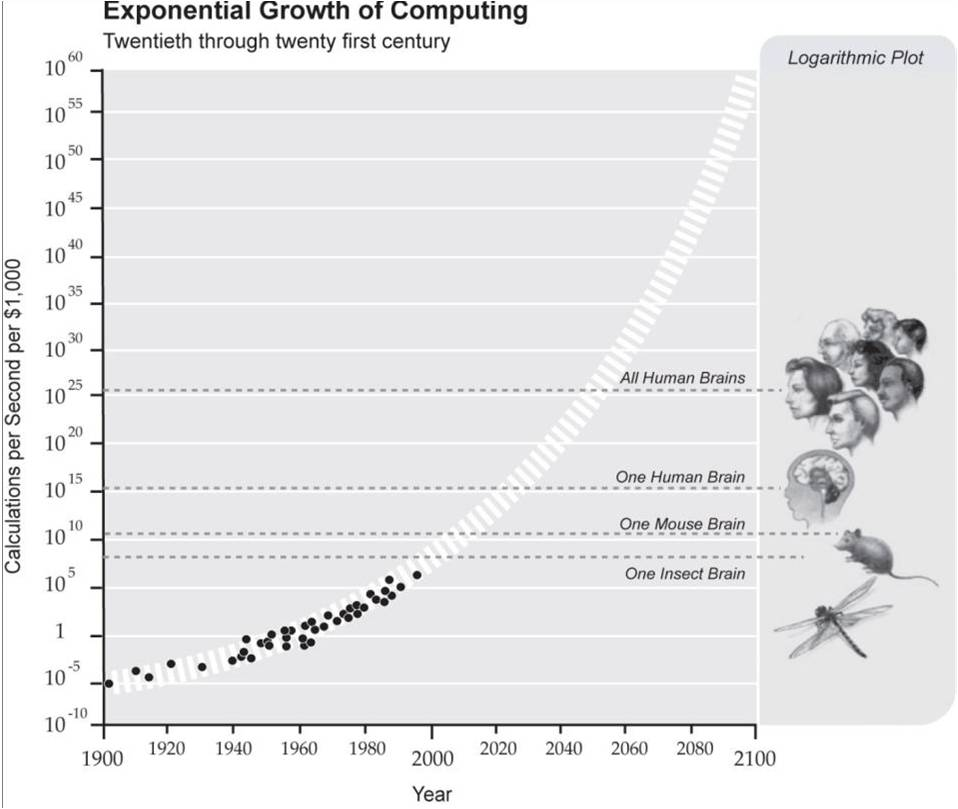
\includegraphics[width=90mm]{plot1.jpg}
  \caption{Estimativa do poder computacional\cite{lawar}\label{overflow}}
\end{figure}

Segundo estudos na área podemos dizer que a média do ser humano é de $10^{16}$ cps.
Um dos melhores super-computadores actuais, o Tianhe-2, supera estes números por pouco, com $3,4\times10^{16}$ cps ocupando $720 m^{2}$, usando 24 MW de energia e custa 347,5 milhões de euros, enquanto que o cérebro ocupa muito pouco e é alimentado por apenas 20 W.
Para termos uma estimativa mais real, recorremos ao preço da média dos computadores pessoais, 900 euros com capacidade de processamento de $10^{10}$ cps.
Recorrendo depois à lei de Moore que diz que a capacidade de processamento aumenta para o dobro a cada dois anos, prevê-se que daqui aproximadamente 10 anos tenhamos uma máquina a um valor aceitável com poder de computação de $10^{16}$ cps.

\subsection{Tornar o software “inteligente”}

Ainda não existe uma solução certa para este problema, apenas debate em volta da mesma. Actualmente existem três estratégias de abordagem para este problema.

\begin{enumerate}
  \item A primeira baseia-se a imitar o comportamento do cérebro, isto porque, quando não se conhece uma maneira de chegar lá, o melhor é aproveitar o exemplo que temos disponível.
Não sendo esta tarefa fácil, tenta-se recorrer a técnicas de reverse engineering para perceber o comportamento do cérebro nas suas operações. Um exemplo desta mímica são as redes neuronais artificiais que já estudámos. Neste caso cria-se uma rede de neurónios que de inicio não têm qualquer informação, mas com o decorrer do tempo as ligações que produzem bons resultados são fortalecidas e as que produzem maus resultados são enfraquecidas. Depois de algo tempo de tentativa e erro é criada um rede que é optimizada para uma certa tarefa.
Outra maneira mais extrema de plagiar o cérebro humano é dividi-lo em camadas, examinar cada uma delas, criar um modelo de cada em software e implementar esse modelo num computador. Se isso for possível teremos um computador capaz de executar as mesmas tarefas que o cérebro humano. Recentemente foi conseguido emular um cérebro com 302 neurónios. O cérebro humano tem 100 mil milhões.
  \item A segunda estratégia consiste em recriar o que a evolução natural fez ao longo dos anos. A motivação desta técnica passa pelo cérebro ser demasiado difícil de recriar, então vamos recriar a evolução que fez que se chegasse a ele.
Para isso, conhecemos os já estudados algoritmos genéticos. Estes baseiam-se em ter vários espécimes que tentam sobreviver num determinado ambiente. Os que têm melhores resultados são procriados entre si e os que têm piores resultados são eliminados. Depois de algum tempo de selecção natural obtém-se um ser, ou neste caso computador, mais inteligente.
O problema desta abordagem é que a selecção natural demora milhares de milhões de anos, mas visto que esta pode ser programada para ir num determinado sentido, diminui em muito este tempo.
  \item A terceira abortarem passa por criar um software num computador, que seja um cientista, que investigue sobre inteligência artificial e em vez de sermos nós a desenvolver o computador, ele desenvolve-se a si mesmo.
\end{enumerate}

Todos estas estratégias parecem estar muito distantes de produzir efeitos práticos, mas tendo em conta a evolução exponencial e as descobertas cientificas que de um momento para o outro mudam a maneira de algo ser feito, esse futuro pode estar bem mais próximo do que pensamos.

\subsection*{E depois da inteligência artificial ultrapassar a inteligência humana?}

Quando a inteligência artificial atingir o nível do cérebro humano, é provável que seja programada para se auto-optimizar e mesmo que não seja, deve ser inteligente o suficiente para o fazer por si. Dessa maneira, o tempo entre ter um computador muito mais inteligente que um humano será muito menor que o tempo decorrido entre hoje e o primeiro computador igual a um cérebro humano. Podemos dizer que vai levar décadas para conseguirmos um sistema de inteligência artificial com o nosso nível de inteligência e depois apenas algumas horas para um nível de inteligência milhares de vezes superior ao humano.

\begin{figure}[ht!]
  \centering
  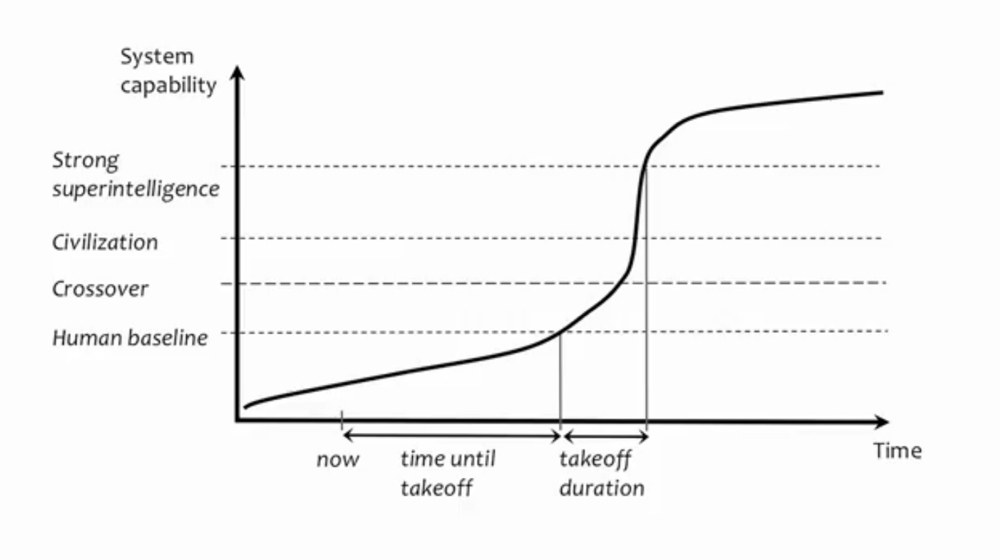
\includegraphics[width=110mm]{plot2.png}
  \caption{Representação da evolução da inteligência artificial comparativamente à inteligência humana\label{overflow}}
\end{figure}

Nessa altura acontecerá uma explosão da inteligência artificial baseada em auto-optimização recursiva. A partir daqui estamos a entrar numa dimensão totalmente diferente que parece retirada de um filme de ficção cientifica, mas que de acordo com cientistas e pensadores relevantes da área é a mais pura das realidades.


\section{Agentes de Super-inteligência Artificial}

Vamos agora aprofundar a super-inteligência artificial pois é essa a que mais problemas (e possíveis benefícios) nos trás. É importante fazermos a distinção no que a super-inteligência artificial diz respeito e classificarmos também dois tipos de super-inteligência.

\subsection{Super-inteligência de velocidade}

Podemos comparar a super-inteligência de velocidade a um supercomputador comparado com um computador normal. Neste caso, estamos perante um agente que consegue pensar muito mais rápido que um humano, mas que pensa da mesma forma.

\subsection{Super-inteligência de qualidade}

Aqui é onde um agente SIA brilha em relação aos humanos. Não só vai pensar muito mais rápido que um humano como também vai pensar de forma muito mais avançada, impossível aos humanos de compreender. A diferença nas super-inteligências é fácil de ver se imaginarmos este cenário: Um chimpanzé a pensar a uma velocidade superior à dos humanos não é suficiente para que seja superior. A evolução fez com que os humanos desenvolvessem capacidades cognitivas que os chimpanzés simplesmente não conseguem percebem, não importa a velocidade do seu cérebro.

O mesmo se passa quando relacionamos um agente SIA com o ser humano, mas a um nível bastante superior, pois esperamos que um SIA possa evoluir muito mais depressa que um humano, pelo que a diferença entre um SIA e um humano possa ser cinco vezes ou mais superior que a diferença entre um humano e uma galinha.

E com isto é bastante importante ressalvar que é impossível sabermos as consequências que um agente SIA irá ter nas nossas vidas e na humanidade. Estamos perante uma bomba relógio que não compreendemos e que só podemos tentar fazer para que expluda da forma mais inócua possível. Segundo Nick Bostrom, filósofo da universidade de Oxford, podemos dividir as consequências de um agente SIA em duas partes distintas. Ou a extinção da humanidade, ou a sua imortalidade.

Até agora, 99,9\% das espécies que viveram na terra extinguiram-se. É natural que os humanos sigam o mesmo caminho. A não ser que isso não aconteça. Bostrom acredita que ainda não houve nada no planeta terra que fosse inteligente o suficiente para atingir a imortalidade, mas que tal não é impossível com um agente SIA\@. O impacto será tão elevado que ou caímos para um lado do espectro ou para outro.

\subsection{Controlo do poder}

Como podemos constatar, quando nos referimos a um agente com super-inteligência estamos a falar de algo com um poder inimaginável. O que acontece se for um grupo com más intenções o primeiro a desenvolver um agente SIA?\@

Na verdade, a comunidade científica não está muito preocupada com este cenário, pois na verdade o problema não está nas intenções dos criadores do agente SIA mas sim no facto desse grupo ter apressado o seu desenvolvimento sem utilizar uma abordagem responsável, levando à perda do controlo sobre o agente SIA\@. Existe sempre o problema de um agente SIA ser criado por um grupo com fins maliciosos, mas qualquer grupo vai ter o mesmo problema em controlar o agente super-inteligente, seja esse grupo bom ou mau.

No entanto, podemos observar a comunidade cientifica dividida em dois quadrantes. Um bastante optimista que vê a chegada de um agente SIA como um sonho tornado realidade e outra parte mais relutante e apreensiva, que teme os efeitos da criação de um agente super-inteligente. Com mais detalhe vamos abordar ambas as visões, e quais as consequências e implicações éticas que o aparecimento de um agente SIA pode ter.

\subsection{Imortalidade e nanotecnologia}

Assumindo que fazemos uma transição pacifica para um SIA, os benefícios para a humanidade são incalculáveis. Ray Kurzweil, inventor conhecido e director de engenharia na Google, está bastante optimista e tem umas visões bastante futuristas.

Na melhor das hipóteses, um SIA resolveria todos os problemas da humanidade. Aquecimento global, cancro, fome, são alguns dos exemplos que um agente super-inteligente poderia resolver. Questões de ética e de filosofia seriam também um tema bastante óbvio para um SIA\@.
Mas mais que isto, e como já tínhamos abordado levemente, um agente SIA pode levar à imortalidade da raça humana. Da mesma forma que um carro com 50 anos continua a andar na estrada enquanto estiver cuidado e com peças substituídas, o mesmo pode acontecer a um humano com o desenvolvimento da nanotecnologia. Na visão de Kurzweil, esse avanço seria possível graças ao aparecimento de um agente super-inteligente. Órgãos substituídos por máquinas super avançadas, células que circulam pelo corpo não necessitando do coração e até cérebros ligados à cloud para nos fazer pensar milhões de vezes mais rápido. Até ao ponto que seremos completamente artificiais. Aqui começam a surgir problemas éticos. Até que ponto continuamos a existir numa máquina apesar de termos a nossa memória e personalidade.

E apesar das previsões de Kurzweil parecerem saídas de um filme de ficção cientifica, a comunidade cientifica não descarta essa possibilidade, mas não tão cedo como Kurzweil afirma. Falaremos nas previsões para estes acontecimentos mais à frente, mas é importante ressalvar que é muito difícil prever com precisão devido a algo chamado enviesamento cognitivo\footnote{dificuldade em acreditar que algo é real até haver uma prova. Um bom exemplo é pensar em quantas pessoas nos anos 80 acreditavam que a Internet iria mudar as suas vidas.}. Mas apesar de existirem bastantes especialistas na área da inteligência artificial a acreditar neste cenário, existe uma outra parte, mais cautelosa no que toca a previsões.

\subsection{Destruição mundial e consciência}

A ficção habituou-nos a este tipo de cenário: Um agente super-inteligente malévolo decide destruir a humanidade. Este cenário retratado no cinema não faz muito sentido na realidade. O bem e o mal são conceitos humanos, e pensar que algo não humano pode perceber estes conceitos é chamado de Antropomorfismo. Como já vimos anteriormente, um SIA destrutivo é possível, mas não por ser malicioso.

Isto levanta outro grande tópico relacionado com a inteligência artificial: a consciência. Será que vamos chegar a ter uma inteligência artificial que consiga rir e sentir as mesmas emoções que nós, ou simplesmente simular essas emoções e essa consciência? Esta questão tem sido explorada dando origem a argumentos como o The Chinese Room\cite{chineseroom}.

Se efectivamente chegarmos a ter humanos artificiais como Kurzweil acredita, será que vamos poder desliga-los como faríamos com um computador ou será visto como um assassinato? Esta é mais uma questão relacionada com a ética quem precisa de ser resolvida.

O problema reside não no facto de se poder criar uma inteligência artificial cujo objectivo é acabar com a humanidade, mas sim no criar uma inteligência artificial criada para cumprir determinada tarefa e que, para a cumprir, acabe com a humanidade ou destrua o mundo como nós os conhecemos. Parece pouco provável mas não é tão diferente do homem matar um animal para comer. O objectivo não é matar o animal mas sim consumir os nutrientes necessários para sobreviver. O animal morrer é efeito colateral do nosso objectivo.

Podemos então observar que um agente autónomo com um objectivo de ``Construir o maior número de casas possíveis da forma mais eficiente possível'' pode facilmente evoluir para matar todos os humanos, de forma a ter mais espaço para construir casas.

O mesmo acontece com o exemplo de programar uma IA com os valores de ``Fazer as pessoas sorrir'' Como estamos a falar de um agente super-inteligente, pode encontrar a melhor maneira com uma neuro-toxina que nos faz paralisar certos músculos da cara para que fiquemos sempre com um sorriso. Está a cumprir com o seu objectivo mas não da maneira como nós queríamos. O mesmo pode acontecer com o ``Acabar com a fome'' em que mata todos os humanos, cumprindo assim o seu objectivo da forma mais eficiente.

E não é só um qi elevado que um agente super-inteligente terá. Bostrom\cite{supint} acredita que um agente SIA terá super poderes como por exemplo:

\begin{description}

  \item[Amplificação de inteligência] \hfill \\
    O agente passa a conseguir aumentar a sua inteligência, tornando-se cada vez mais inteligente
  \item[Estategização] \hfill \\
    O agente passa a conseguir conceber e analisar planos a longo prazo
  \item[Manipulação social] \hfill \\
    O agente tem um poder de persuasão bastante elevado
  \item[Outros] \hfill \\
    hacking, investigação tecnológica e habilidade de ganhar dinheiro através do sistema financeiro serão também especialidades do agente SIA

\end{description}

Mas ainda assim o problema estará na transição. Se não conseguirmos planear bem o objectivo do agente de inteligência artificial geral, quando este evoluir para SIA, o espectro do plano vai alterar por completo. Cabe-nos a nós conter o máximo possível o agente geral, pois é-nos impossível fazer o mesmo com um agente SIA, devido aos poderes que possuí. Não nos podemos esquecer que um agente SIA é anos-luz melhor que qualquer humano.

São inúmeros os problema que enfrentamos com o aparecimento de agentes super-inteligentes. Tanta gente a querer desenvolver o primeiro SIA que certas questões importantes podem não ser tomadas em conta. Os efeitos podem ser destrutivos e podemos não ter tempo para reagir. É isso que faz mover os especialistas na área, mas será que conseguimos resolver todos os problemas até ao seu aparecimento?

\section{Previsão para o aparecimento de um agente SIA}

Existem várias previsões para o aparecimento de um SIA, mas onde uma grande maioria dos cientistas estão de acordo é que primeiro: O surgimento da super-inteligência é inevitável e segundo: este acontecimento vai ter lugar no século XXI\@.

Fazendo uma média bastante por alto de previsões e alguns dos questionários feitos a especialistas da área da inteligência artificial, estamos perante os seguintes números:

\begin{itemize}

  \item 2040 - Aparecimento do primeiro agente de inteligência artificial equiparado ao humano
  \item 2060 - Aparecimento do primeiro agente de super-inteligência artificial

\end{itemize}

Estas datas estão bastante próximas de nós mas podem parecer inexequível para alguém fora da área. Olhando para trás no tempo, e comparando o desenvolvimento de três séculos: X, XV e XX, a diferença entre o século XV e XX é muito superior à diferença entre o século X e XV\@.

Não estamos portanto a falar de um crescimento linear mas de um crescimento exponencial. Tal como a lei de Moore, que também aponta um crescimento exponencial para o número de transístores num circuito integrado, também aqui, utilizando aquilo a que Kurzweil chama de lei de rendimentos acelerados
(law of accelerating returns), expandindo assim a lei de Moore a outras tecnologias e naturalmente, a todo o desenvolvimento tecnológico. Segundo esta lei, ao ritmo do desenvolvimento do século XXI, o inteiro desenvolvimento do século XX demoraria apenas 20 anos. Mais ainda, durante o século XXI podemos vir a ter um progresso 1000 vezes superior ao século XX\@. Se Kurzweil e aqueles que concordam com ele estiverem certos, o mundo em 2050 pode ser completamente diferente do mundo que conhecemos hoje, ao ponto da diferença ser tão grande como se alguém de 1700 viajasse para 2015. Se pensarmos desta forma, talvez as datas de 2040 e 2060 para inteligência artificial geral e super-inteligência não pareça tão descabido.

A verdadeira revolução está a chegar, e se, por um lado pode resolver todos os nosso problemas, por outro pode acabar com todos os problemas de uma só vez. Por isso é que os especialistas chamam à super-inteligência a última invenção da humanidade, e o ultimo desafio que vamos enfrentar.

\begin{thebibliography}{4}

  \bibitem{FLI} Future of Life Institute, \url{http://futureoflife.org/misc/AI}
  \bibitem{gates} Reddit Ask me Anything, \url{http://www.reddit.com/r/IAmA/comments/2tzjp7/hi_reddit_im_bill_gates_and_im_back_for_my_third/co3r3g8}
  \bibitem{hawking} BBC News, \url{http://www.bbc.com/news/technology-30290540}
  \bibitem{chineseroom} Chinese Room - Stanford Encyclopedia of Philosophy, \url{http://plato.stanford.edu/entries/chinese-room/}
  \bibitem{vfdebate} Vanity Fair, \url{http://www.vanityfair.com/news/tech/2014/11/artificial-intelligence-singularity-theory}
  \bibitem{supint} Nick Bostrom:
    Superintelligence: Paths, Dangers, Strategies
    Oxford University Press (2014)
  \bibitem{supint2} Nick Bostrom:
    How Long Before Superintelligence?
    Oxfrord Future of Humanity Institute (1997)
  \bibitem{aipf} Moshe Y. Vardi:
    Artificial Intelligence: Past and Future
    Communications of the ACM, (2012)
  \bibitem{failai} Stuart Armstrong, Kaj Sotala:
    How We’re Predicting AI—or Failing To
    Machine Intelligence Research Institute (2012)
  \bibitem{lawar} Ray Kurzweil:
    The Law of Accelerating Returns,
    \url{http://www.kurzweilai.net/the-law-of-accelerating-returns}
  \bibitem{sing} Ray Kurzweil:
    The Singularity Is Near: When Humans Transcend Biology
    Viking, (2005)

\end{thebibliography}

\end{document}
